\section{Ad-hoc сети}

В век коммуникационных устройств, социальных сетей и прочих сервисов, сообщение на расстоянии и мгновенный обмен информацией кажутся чем-то само собой разумеющимися. Однако возможность оставаться на связи именно в те моменты, когда коммуникационная инфраструктура оказывается нарушенной, приобретает особое значение. В подобных случаях все более привлекательным вариантом становится создание беспроводной самоорганизующейся (или ad hoc) сети. Такая структура формирует сама себя всякий раз, когда специально запрограммированные устройства связи оказываются в пределах прямого доступа. Каждое из них выполняет в динамической сети функции и передатчика, и приемника, а также, что очень важно, служит ретрансляционным пунктом для всех ближайших приспособлений. Устройства, расстояние между которыми превышает дальность прямой связи, могут поддерживать связь между собой. Таким образом, каждый узел в сети служит и коммуникатором для собственных сообщений, и элементом инфраструктуры для сообщений других узлов.

Когда вы звоните другу по мобильному телефону, в беспроводной связи задействован только каждый из соединяемых телефонов и ближайшая к нему
вышка сотовой связи. Вышки неподвижны и связаны между собой обширной сетью проводов и кабелей. В беспроводных локальных сетях, в частности Wi-Fi, также используются неподвижные антенны и проводные соединения. Такой подход имеет как достоинства, так и недостатки. Однако использование фиксированной инфраструктуры делает эти сети уязвимыми: их работа нарушается в случае отключения электропитания и других сбоев даже при исправности отдельных телефонов и других мобильных устройств в зоне действия сети.

Надежность динамических сетей намного выше. Ad-hoc сети предлагают уникальные преимущества и универсальность для определенных условий и для определенных приложений. Так как нет фиксированной инфраструктуры, базовых станций, то такие сети могут быть созданы и использоваться в любое время и в любом месте. Управление компьютерной сетью усложняется следующими факторами:
\begin{enumerate}
\item Необходимость экономии электроэнергии портативных устройств приводит к значительному снижению радиуса действия приемо-передающих блоков.
\item Радиус действия снижается также за счет естественных и искусственных препятствий, имеющихся на территории.
\item Малый радиус действия приводит к риску потери связанности сети и невозможности оперативной передачи информации между компонентами.
\item На фактор связанности влияют также перемещения узлов сети на местности.
\end{enumerate}

Разработка таких сетей ведется уже больше трех десятилетий, но лишь в последние годы успехи теории сетей привели к созданию первых рабочих крупномасштабных систем. Для того, чтобы подобные сети получили широкое распространение, требуется еще ряд технических прорывов, но на нескольких направлениях успехи уже достигнуты. В качестве основного формального представления такой сети используется геометрический граф. Ребро между двумя узлами сети существует тогда и только тогда, когда расстояние между ними меньше или равно радиусу покрытия этих узлов.

Важным обстоятельством беспроводной самоорганизующейся сети является то, что узлы могут включаться и выключаться из нее в любой момент, что предопределяет случайный характер структуры сети. Именно из этого фактора вытекает необходимость анализа структуры беспроводной сети (геометрического графа) на наличие мостов, путей, маршрутов, компонент связности, циклов и других важных характеристик графа по первому запросу пользователя. При этом результат на запрос должен быть предоставлен как можно быстрее. Для решения этой задачи нами было принято решение о создании программного комплекса вероятностного моделирования ad-hoc сети.

\section{Система вероятностного моделирования ad-hoc сетей}

Для упрощения моделирования и анализа работы системы, а так же для возможности ее расширения было решено придерживаться сервис-ориентированной архитектуры программы, то есть клиент-сервис. Приложение предполагает динамическое подключение библиотек с алгоритмами, что позволит дополнять функционал приложения. Как и во всех приложений такого типа, ресурсоемкие вычисления предполагается проводить на стороне сервера, клиент только оставляет запрос на выполнения определенного алгоритма и ожидает результат.

Программный комплекс состоит из четырех основных частей:
\begin{enumerate}
\item Веб-клиент. Часть, благодаря которой, пользователь сможет подавать запросы на вычисление определенных данных на множестве сетей и получать результаты. Структура клиента генерируется при запуске в зависимости от доступных алгоритмов, что позволяет использовать избавить пользователя от возможных проблем с использованием недоступных на тот момент алгоритмов; 
\item Менеджер заданий. Отвечает за анализ запросов и их дальнейшую обработку, взаимодействует с базой данных и менеджером алгоритмов. Если запрашиваемые данные уже имеются в базе данных, то они сразу отправляются пользователю. В противном случае, данный запрос поступает к менеджеру алгоритмов, и ждет вычисления результатов;
\item Менеджер алгоритмов. Анализирует полученный запрос, после чего запускает необходимый алгоритм на запрашиваемых данных. Время вычислений оптимизируется за счет использования ресурсов, имеющихся на данном компьютере (многопоточность, использование cuda-вычислений);
\item Веб-сервис. Обеспечивает взаимодействие веб-клиента и менеджера заданий, ставя в очередь на выполнения запросы, получаемые от клиента. Так же анализирует информацию о доступных алгоритмах, предоставляемую менеджером алгоритмов, передавая ее веб-клиенту.  
\end{enumerate}
Общая схема проекта представлена на рисунке \ref{structure}.

\begin{figure}[ht]
\center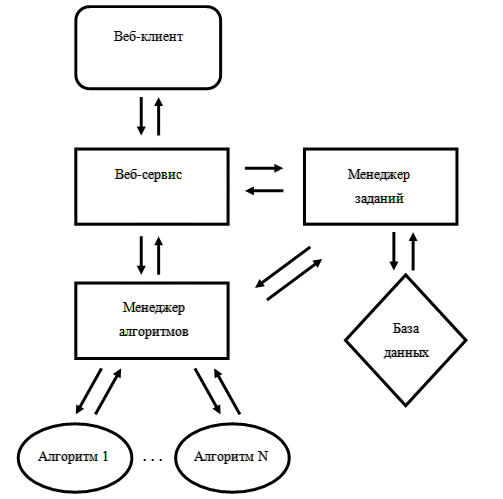
\includegraphics[width=0.8\textwidth]{structure}
\caption{Схема системы вероятностного моделирования ad-hoc сетей}\label{structure}
\end{figure}

Данный проект был дан на реализацию четырем студентам (по количеству частей системного комплекса). Мной было решено реализовывать первую часть описанного программного комплекса – веб-клиент. 